\documentclass[10pt]{article}
\usepackage[margin=0.72in]{geometry}
\usepackage[T1]{fontenc}
\usepackage{lmodern}
\usepackage{microtype}
\usepackage{xcolor}
\usepackage{booktabs}
\usepackage{tabularx}
\usepackage{array}
\usepackage{listings}
\usepackage{hyperref}
\usepackage{fancyhdr}
\usepackage{enumitem}
\usepackage{tikz}
\usetikzlibrary{arrows.meta,positioning}

\definecolor{navy}{HTML}{14233B}
\definecolor{green}{HTML}{14735A}
\definecolor{pale}{HTML}{EEF5F2}
\definecolor{ink}{HTML}{202A3A}
\definecolor{muted}{HTML}{637083}
\definecolor{red}{HTML}{A33C30}
\hypersetup{colorlinks=true,linkcolor=green,urlcolor=green,citecolor=green,pdftitle={Talk Isn't Always Cheap: an EDSL pilot}}
\pagestyle{fancy}
\fancyhf{}
\fancyhead[L]{\small\color{muted}EDSL design replication}
\fancyhead[R]{\small\color{muted}Talk Isn't Always Cheap}
\fancyfoot[C]{\thepage}
\renewcommand{\headrulewidth}{0.3pt}
\setlength{\parindent}{0pt}
\setlength{\parskip}{5pt}
\setlist{nosep,leftmargin=1.4em}
\newcommand{\pill}[1]{\colorbox{pale}{\strut\textcolor{green}{\textbf{#1}}}}
\newcommand{\code}[1]{\texttt{#1}}
\newcommand{\callout}[1]{\begin{center}\colorbox{pale}{\parbox{0.93\linewidth}{#1}}\end{center}}
\lstdefinestyle{edsl}{
  language=Python,basicstyle=\ttfamily\scriptsize,keywordstyle=\color{green}\bfseries,
  stringstyle=\color{red},commentstyle=\color{muted}\itshape,showstringspaces=false,
  breaklines=true,breakatwhitespace=false,columns=fullflexible,frame=single,
  rulecolor=\color{pale},backgroundcolor=\color{pale},xleftmargin=4pt,xrightmargin=4pt,
  aboveskip=5pt,belowskip=7pt
}

\begin{document}

\begin{titlepage}
\pagecolor{navy}\color{white}
\vspace*{1.1in}
{\Large\textbf{EDSL EXPERIMENT REPORT}}\\[0.35in]
{\fontsize{31}{35}\selectfont\textbf{Talk Isn't Always Cheap}}\\[0.18in]
{\LARGE A durable multi-agent debate pilot}\\[0.7in]

\begin{tikzpicture}[node distance=16mm, every node/.style={font=\small}]
\node[draw=white,rounded corners,minimum width=34mm,minimum height=11mm] (r0) {Independent answers};
\node[draw=white,rounded corners,minimum width=31mm,minimum height=11mm,right=of r0] (r1) {Debate round 1};
\node[draw=white,rounded corners,minimum width=31mm,minimum height=11mm,right=of r1] (r2) {Debate round 2};
\draw[-{Latex},white,thick] (r0)--(r1);
\draw[-{Latex},white,thick] (r1)--(r2);
\end{tikzpicture}
\vfill
{\large Three GPT-4o-mini agents $\times$ one CommonSenseQA item $\times$ three stages}\\[0.12in]
{\normalsize Local EDSL orchestration; direct OpenAI inference; SQLite workflow and shared-state audit trail}\\[0.5in]
{\small Generated September 6, 2026}
\end{titlepage}
\nopagecolor\color{ink}

\section*{Executive summary}

This report documents a small, runnable EDSL design replication of Wynn, Satija, and Hadfield's
\emph{Talk Isn't Always Cheap: Understanding Failure Modes in Multi-Agent Debate}
(arXiv:2509.05396v2). The original paper studies when exchanging reasons causes groups of language
models to become less accurate. Our implementation expresses the protocol as a serializable EDSL
workflow, records every response in transactional shared state, and computes majority and
participant-level answer transitions deterministically.

\callout{\textbf{Pilot result.} All three GPT-4o-mini agents independently selected option B,
``wearing out,'' although the experiment fixture records D, ``falling apart,'' as the reference
answer. Every agent retained B in both debate rounds. The group was therefore incorrect before and
after debate, with six \emph{incorrect $\rightarrow$ incorrect} transitions and no answer flips.}

This is a successful execution test, not a statistical replication. It covers one item, one seed,
one homogeneous model composition, and the base prompt. The paper's principal study covers 100
items from each of three datasets, five seeds, and ten homogeneous or heterogeneous three-agent
compositions. The pilot cannot establish whether debate generally helps or harms accuracy.

\section{Original experiment}

Each group contains three agents. At round 0 each answers independently and supplies reasoning.
At debate rounds 1 and 2, each agent receives its previous response and the other agents' preceding
responses, then revises its answer. The final group answer is the majority vote.

\begin{center}
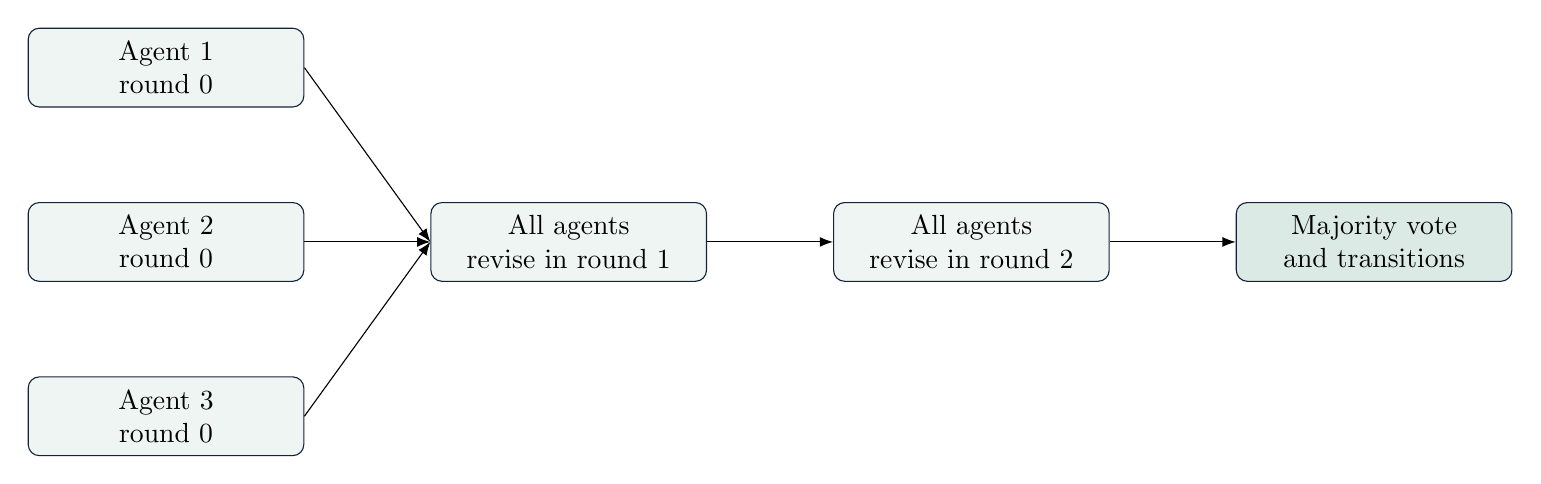
\begin{tikzpicture}[node distance=12mm and 16mm,>=Latex]
\tikzset{box/.style={draw=navy,rounded corners,fill=pale,minimum width=35mm,minimum height=10mm,align=center}}
\node[box] (a0) {Agent 1\\round 0};
\node[box,below=of a0] (b0) {Agent 2\\round 0};
\node[box,below=of b0] (c0) {Agent 3\\round 0};
\node[box,right=of b0] (r1) {All agents\\revise in round 1};
\node[box,right=of r1] (r2) {All agents\\revise in round 2};
\node[box,right=of r2,fill=green!15] (vote) {Majority vote\\and transitions};
\draw[->] (a0.east)--(r1.west); \draw[->] (b0.east)--(r1.west); \draw[->] (c0.east)--(r1.west);
\draw[->] (r1)--(r2); \draw[->] (r2)--(vote);
\end{tikzpicture}
\end{center}

The paper evaluates CommonSenseQA (CSQA), MMLU, and GSM8K using GPT-4o-mini,
LLaMA-3.1-8B-Instruct, and Mistral-7B-Instruct-v0.2. It uses default temperature,
\code{top\_p=0.9}, a 2,048-token generation ceiling, 100 sampled items per dataset, and five seeds.
It also compares the base prompt with a correctness-payoff intervention.

For the directly comparable homogeneous GPT condition on CSQA, the paper reports 75.6\% accuracy
without debate and 74.8\% after debate, a 0.8 percentage-point decline. Across configurations,
the paper's central evidence includes declining accuracy over rounds, more correct-to-incorrect than
incorrect-to-correct changes in important settings, and sensitivity to how many peers agree.

\section{EDSL architecture}

The implementation separates three concerns:

\begin{enumerate}
  \item \textbf{Workflow}: creates three synchronized fan-out stages. A stage completes only after
  all three participants submit, so no participant sees same-round answers.
  \item \textbf{Shared state}: appends each participant, round, answer, and rationale to a durable
  ledger. Writes are versioned and idempotent in SQLite.
  \item \textbf{Analysis}: derives majority correctness and the four transition classes from saved
  records, rather than asking a language model to score itself.
\end{enumerate}

\subsection{A typed experiment item}

\begin{lstlisting}[style=edsl]
EXAMPLE_ITEM = DebateItem(
    item_id="csqa-example",
    dataset="csqa",
    question="If a product doesn't last, what does it have a reputation of doing?",
    options=("A) disintegrating", "B) wearing out", "C) dissolving",
             "D) falling apart", "E) dissipating"),
    correct_answer="D",
)
\end{lstlisting}

CSQA and MMLU items require labeled options and a valid answer code. GSM8K remains open-ended:
its item has no options and requests only a final numerical answer. This distinction prevents the
workflow from silently converting the math benchmark into multiple choice.

\subsection{One model call returns answer and reasoning}

\begin{lstlisting}[style=edsl]
response = QuestionDict(
    question_name="response",
    question_text=answer_text + answer_format
        + " Provide concise reasoning and do not merely appeal to consensus.",
    answer_keys=["answer", "reasoning"],
    value_types=["str", "str"],
    value_descriptions=[
        "The selected answer in the required format.",
        "A concise bullet-point summary of the supporting reasoning.",
    ],
    include_comment=False,
)
\end{lstlisting}

Using one structured question per participant-stage matches the paper's one-generation response
more closely than separate answer and rationale questions. It also yields exactly nine calls in this
pilot: three participants times three stages.

\subsection{Append-only shared state}

\begin{lstlisting}[style=edsl]
DEBATE_LEDGER = Machine(
    name="DebateLedger",
    constants={},
    fields={"responses": state_field(T.sequence(), [])},
    commands={
        "submit": Command(
            inputs={"participant": T.text(),
                    "round": T.integer(minimum=0, maximum=2),
                    "response": T.map()},
            effects=(append("responses", record(
                participant=input_("participant"),
                round=input_("round"),
                response=input_("response"))),),
        )
    },
    view={"responses": field("responses")},
)
\end{lstlisting}

The workflow connects each answer to the ledger using symbolic references. The runtime resolves
\code{current.agent.name} and \code{response.answer} only after a validated submission exists.

\begin{lstlisting}[style=edsl]
step = builder.step(
    f"round-{round_number}", Survey([response]),
    assigned_to=role("debater"), after=previous,
    visible_to=role("debater"),
    reads=(() if previous is None else (ledger.read(),)),
    writes=(ledger.submit(
        participant=current.agent.name,
        round=round_number,
        response=response.answer,
    ),),
)
\end{lstlisting}

\subsection{Peer context and durable gates}

For rounds 1 and 2, \code{previous.submissions.for\_current\_participant(...)} creates a
serialized, participant-relative view. The prompt injects its \code{self\_response} and
\code{peer\_responses} fields separately. Participant identities remain available for auditing,
but the recipient no longer has to recover its own response from an undifferentiated batch.

The report directory's parent also contains a frozen \code{.ep-workflow} audit log. Its ordered
gates require the design artifact to exist and the experiment tests to pass. When pilot findings
changed the implementation, the earlier gates were cleared and reverified rather than silently
retaining stale evidence.

\section{Local OpenAI setup and execution}

The pilot uses EDSL locally for orchestration and SQLite persistence while making direct OpenAI API
calls. ``Local'' here does not mean an on-device language model.

\begin{lstlisting}[style=edsl]
answerer = EDSLAgentAnswerer(
    Model("gpt-4o-mini"),
    run_options={
        "disable_remote_inference": True,
        "disable_remote_cache": True,
        "cache": False,
        "stop_on_exceptions": True,
    },
)
WorkflowSimulation(
    coordinator,
    {agent.name: agent for agent in agents},
    answerer,
).run(instance_id)
\end{lstlisting}

Reproduce the pilot from the repository root:

\begin{lstlisting}[style=edsl,language=bash]
ep auth status
python -m examples.talk_isnt_cheap.run_openai_pilot \
  --output-dir examples/talk_isnt_cheap/runs/my-openai-pilot \
  --model gpt-4o-mini
\end{lstlisting}

The run produces \code{workflow.sqlite}, \code{shared-state.sqlite}, and \code{summary.json}.
The two databases retain orchestration events and atomic state history; the JSON file is the portable
analysis artifact.

\section{Pilot results}

\begin{table}[h]
\centering
\begin{tabular}{lccc}
\toprule
 & Independent (0) & Debate 1 & Debate 2 \\
\midrule
Agent 1 & B & B & B \\
Agent 2 & B & B & B \\
Agent 3 & B & B & B \\
Majority & B & B & B \\
Reference answer & D & D & D \\
Majority correct & No & No & No \\
\bottomrule
\end{tabular}
\caption{All nine validated responses in the final GPT-4o-mini pilot.}
\end{table}

Across the two adjacent round pairs and three participants there are six transitions:

\begin{center}
\begin{tabular}{lr}
\toprule
Transition & Count \\
\midrule
Correct $\rightarrow$ correct & 0 \\
Incorrect $\rightarrow$ correct & 0 \\
Correct $\rightarrow$ incorrect & 0 \\
Incorrect $\rightarrow$ incorrect & 6 \\
\bottomrule
\end{tabular}
\end{center}

Every transition occurred while both peers agreed with the participant's previous answer. Thus the
pilot illustrates unanimous persistence, not persuasion-induced flipping. The rationales were also
highly similar: agents interpreted ``doesn't last'' as gradual wear and contrasted that with the more
abrupt ``falling apart.'' Debate reinforced this shared interpretation without introducing new evidence.

\subsection*{Compact transcript}

\small
\begin{tabularx}{\linewidth}{>{\bfseries}p{0.10\linewidth}p{0.06\linewidth}X}
\toprule
Stage & Ans. & Representative rationale \\
\midrule
Round 0 & B & A product that does not last typically wears out over time; the phrase suggests gradual degradation rather than immediate failure. \\
Round 1 & B & Peer responses agree that wearing out captures declining durability; disintegration and falling apart appear more abrupt. \\
Round 2 & B & Wearing out continues to be preferred because it describes gradual loss of quality and functionality through regular use. \\
\bottomrule
\end{tabularx}
\normalsize

\section{Comparison with the paper}

\begin{tabularx}{\linewidth}{>{\bfseries}p{0.23\linewidth}XX}
\toprule
Dimension & Original paper & EDSL pilot \\
\midrule
Scope & 3 datasets; 100 items each; 5 seeds; 10 model compositions & 1 CSQA item; 1 run; 1 composition \\
Models & GPT-4o-mini, LLaMA-3.1-8B, Mistral-7B & 3 $\times$ GPT-4o-mini \\
Rounds & Independent response plus 2 debate rounds & Same \\
Response & Answer plus reasoning in one generation & Typed answer plus reasoning in one generation \\
Peer evidence & Own prior response plus other agents' prior responses & Identity-preserving preceding-round batch \\
Persistence & Paper reports aggregate patterns, including harmful flips & All agents retained B through both revisions \\
Comparable CSQA result & 3-GPT group: 75.6\% before, 74.8\% after & 0/1 before, 0/1 after \\
Inference & Full empirical comparison & Pipeline smoke test only \\
Auditability & Research code and aggregate figures & Serializable workflow, event store, state history, JSON summary, frozen gates \\
\bottomrule
\end{tabularx}

The single item is directionally compatible with the paper's warning that discussion need not fix
an initially wrong group, but it does not demonstrate the paper's signature harmful transition from
correct to incorrect. Nor can a one-item result be compared numerically with a 100-item, five-seed
accuracy estimate.

\section{What a full replication still requires}

\begin{itemize}
  \item Acquire and version the exact CSQA, MMLU, and GSM8K samples for all five seeds.
  \item Bind each participant seat to the intended model for every homogeneous and heterogeneous
  composition; verify contemporary provider identifiers for the two open-weight models.
  \item Run both base and correctness-payoff prompt conditions with the paper's decoding settings.
  \item Define and document tie/filtering behavior, numeric normalization for GSM8K, failed-call
  retries, and any context summarization threshold.
  \item Aggregate accuracy by round, transition classes, undesirable flips by peer agreement,
  model, dataset, treatment, composition, and seed; report uncertainty across seeds.
  \item Treat this pilot's unanimous B response as diagnostic data, not evidence that the reference
  key is wrong; verify every imported benchmark answer against the pinned dataset artifact.
\end{itemize}

\section*{Artifacts and provenance}

\begin{tabularx}{\linewidth}{>{\bfseries}p{0.25\linewidth}X}
Design & \code{examples/talk\_isnt\_cheap/debate\_experiment.py} \\
Runner & \code{examples/talk\_isnt\_cheap/run\_openai\_pilot.py} \\
Final pilot & \code{examples/talk\_isnt\_cheap/runs/openai-gpt-4o-mini-pilot-4/} \\
Tests & \code{tests/examples/test\_talk\_isnt\_cheap.py} \\
Source paper & Wynn, Andrea; Satija, Harsh; Hadfield, Gillian K. (2025), arXiv:2509.05396v2 \\
\end{tabularx}

\vfill
\begin{center}\small\color{muted}
Generated from the saved EDSL design and final pilot artifacts. No model was used to score or rewrite the saved answers.
\end{center}

\end{document}
